
% Macros for character names
% Should probably move to the actual fiction chapter
\newcommand{\salesjerk}[0]{Levi}

\chapter{AI can be Jerks: Learning from the Best}

The previous story saw our protagonist start her carrer, and our
essays will also begin with foundational material: what a lay user needs
to understand what's happening in the story and how realistic it is.
We'll save the more fanciful and complicated stuff for later chapters.

For the moment, we focus on a facet of artificial intelligence called
machine learning.  Machine learning is a small subset of artificial
intelligence,\footnote{Research is organized around conferences; these
  onferences often form a community that is protective of its turf.
  While there is substantial overlap between the communities (e.g.,
  the Neural Information Processing Systems conference), many machine
  learning researchers (e.g., the International Conference on Machine
  Learning) prefer to remain distinct from ``pure'' artificial
  intelligence.} but unlike much of the fancifal claims of aritificial
intelligence prophets, it actually works \emph{now}.

We first introduce a key component of machine learning---objective
functions---that define why systems act they way they do. We then show
how bad human behavior can be mimicked by these algorithms (it's
already happening!).  Finally, we close the chapter with a call to
action: keep your computers safe!

\section{Learning by Doing: Objective Functions}
\label{sec:objective-functions}

Let us begin with an essential and underappreciated example of machine
learning that simply works and makes modern life liveable: spam
filters.  An e-mail is either spam or not; computers think in ones and
zeros, so let's call spam a one and not spam a zero.

An algorithm does not just say ``yes'' or ``no'' to whether an e-mail
is spam.  It typically gives a score for each e-mail: the higher the
score, the more confident it is the e-mail is spam.  For the moment,
let's assume that all of the numbers are between zero and one (e.g.,
they are a probability).

A perfect score would be if all spam e-mails got a 1.0 and all of the
good e-mails got 0.0.  Both perfection and absolute certainty are
unattainable goals, so we need to deal with both errors and
uncertainty.  So we sum all of the spam documents---how far the
scores are from 1.0---and we sum all of the good e-mails---how
far the scores are from 0.0.  This sum is our \emph{objective
  function}: a perfect score is 0.0 and the worst score is the number
of e-mails.

Machine learning algorithms are defined by \emph{parameters}.  For
example, a parameter might define what the algorithm does when it sees
the word ``viagra'' or the phrase ``I am a Nigerian prince''.  These
parameters effectively define the algorithm; machine learning
algorithms learn how to set these parameters from data, a process that
can take multiple names,\footnote{Some of the alternate names are
  field specific; for example, in statistics this is called inference
  and the objective function is typically called the likelihood.
  However, the mechanics are similar.  For some applications, it's
  called a ``loss function'', but we'll stick with the more general
  term.} but we'll call it ``optimization''.

\subsection{Optimization}

Optimization is the process where machine learning uses data to find
the parameters that give the best score on the objective function.
Typically, the process starts with a random setting of the parameters.
This will do \emph{horribly}, but it provides a place to start: the
early improvements will be easy.

The learning process will slowly change the parameters to ever so
slightly improve the objective function.\footnote{Mathematically, this
  is usually by looking at the derivative (if you remember that from your calculus class) of the objective function with
  respect to the parameters.}  The learning process goes document by
document to slowly improve the objective function.  Eventually, modern
optimization techniques find a setting of the parameters that work
well for this problem.\footnote{The form of the objective function
  determines whether this answer will be the best possible or merely a
  ``good'' solution.}

Let's take a concrete example.  Let's say that this is the first
e-mail the algorithm has seen with the phrase ``special offer'' and the algorithm says that it
is spam with score 0.7.  This is a spam e-mail, so the algorithm could
do better in terms of its objective function if the parameter
associated with the phrase ``special offer'' were more strongly
associated with spam.  So our optimization will push the parameter a
little more in that direction so that the score is 0.75 the next time
it sees a similar document.  This continues until the parameters
cannot get any better.

All of this seems fairly straightforward, but there is some art to
creating these systems.  Defining the parameters requires a bit of
expertise: either hand-crafting parameters that fit the problem well
or using automatic approaches that learn effective representations.
Doing this well requires quite a bit of work, and often your first
(and second, etc.) attempt will usually fail.

\subsection{Is this Artificial Intelligence?}

A reasonable question is whether this is \emph{intelligence}.  Before
we get into the nuance of the question, the answer---given the systems
we have discussed---is definitely \textbf{no}.  But because we'll
discuss things that \emph{are} artificial intelligence later in the
book, it's useful to discuss what it means for a system to be
intelligent now.  This way, we can at least see why these systems are
not intelligent.

In some ways, impressive achievements in technology is a moving
target.  After a few decades of living with machines that do a
formerly impressive task, we cease to be impressed by it and its
comparison to humans.\footnote{This is not just for intelligence;
  \song{The Ballad of John Henry} celebrates a competition between a
  steam drill and ``a man who ain't nothing but a man\dots with a
  hammer in [his] hand.''  Today, such comparisons and competitions
  seem silly.}  The luster of adding machines has faded into beige
quotidian boringness through the twentieth century.

Even in my own life, my excitement about halfway decent speech
recognition---taking a stream of speech and transcribing it into words
on a screen---has given way to annoyance at my phones' (increasingly
rare) mistakes.  Both of these were considered tasks that only humans
could do\footnote{The term ``computer'' originally referred to
  specially trained humans proficient at high-stakes, accurate
  calculations.  \citet{light-99} documents how labor shortages during
World War II increasingly a female profession.  However, like the
protagonists of \book{Hidden Figures} by Margot Lee Shetterly, the
women remain in the background.} but now are so ubiquitous that half of humanity is
joined at the hip to devices that do both these things.

A skeptic would say that machine learning is a mere mechanical
mathematical exercise.  The algorithm that decides whether an e-mail
is spam or not doesn't actually understand what it's reading, and the
parameters were defined by a human.  While the values of the
parameters come from data, there's no real learning going on.

A proponent would counter that intelligence is actually a combination
of many smaller processes.  To understand an e-mail, we need to
understand parts of speech, syntax, discourse, and pragmatics.  Each
of these can be thought of as individual problems like spam
classification.  Each one is mechanistic, but together they form a
process that can be viewed as intelligent.

For the moment, we will leave the debate there.
Chapter~\ref{chap:gai} takes up the question about what it means to be
intelligent and how to measure the intelligence of algorithms.

\TODO{tone this down}

Nevertheless, machine learning has earned the reputation of being
``artificial intelligence that works''.  Its mechanistic definition is
a virtue: it is easy to see what works and what does not.  Just as the
objective function allows the algorithm to tune individual parameters
to improve a single task, the clear defintion allows researchers to
tweak problems, models, and data to get better at important tasks.

Machine learning has dones well at many tasks: identifying objects in
a picture~\citep{russakovsky-15}, playing
games~\citep{vinyals2017starcraft}, answering
questions~\citep{ferruci-10}, and driving cars~\citep{thrun-10}.
%
These tasks are impressive, but each task is a composition of smaller objective
functions.
%
As we move into ``real'' artificial intelligence, these objective
functions will play an outsized role.
%
While the underlying mechanism here is relatively dumb, it is worth
grappling with the important questions of defining a good objective
function.

\subsection{}

In our example in \crunchyCity{}, the objective function is typically
aligned with business goals.
%
For \energyCompany{}, this could be the number of new subscribers,
revenue, or profits.
%
Other companies have different objectives:
many web sites optimize engagement~\citep{hoiles-17}, while logistics
companies want to minimize travel time given promises made to customers~\citep{fiat-16}.



\subsection{Training Data}

This machine learning setup,\footnote{Formally, this setup is called
  \emph{supervised machine learning}, where there are specific
  input--output examples the algorithm must replicate.  Unsupervised
  machine learning is another active area of research, but it is much
  harder to see when things are working well.  We talk about
  applications and evaluations of unsupervised machine learning in
  Section~\ref{sec:unsup}} however, only works with generous training
data.  Modern machine learning algorithms are also notoriously data
hungry.  They can always do better, but they can only do better at the
cost of additional training data: if you see input~$x$, what should
your output~$y$ be?

However, many tasks can be framed as mechanical calculations; they
do not require abstract reasoning or generalization what people today
consider ``intelligence''.  More specifically, they requires hundreds
or thousands of examples to know what to do.  \energyJerk{} is a
prolific demonstrator of what (not) to do.  A human could learn
\energyJerk{}'s tricks from a high-level description.  An algorithm
learns to copy. 

This simple mimicry can seem sophisticated.  It's couched in terms
that sound sophisticated but only facilitate superficial copying
(Figure~\ref{fig:la-ml}).  \energyCompany{} has a relatively simple
objective function to optimize: are people buying its
software or not?  If sales go up, it's good.  If sales go down, it's
bad.  Optimizing this function without any help is a difficult problem
(this is why \textsc{ceo}s are paid so much), but \energyCompany{}
doesn't have to do it alone: it learned it from \energyJerk{}.

\begin{marginfigure}%
  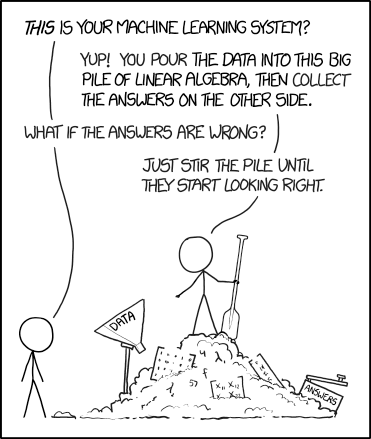
\includegraphics[width=\linewidth]{figures/xkcd-la-ml}
  \caption{Much of ``Machine Learning'' is copying in the form of
    complicated equations defined by mathematical formulas using fancy
    words like ``linear algebra'', ``gradients'', and ``nonconvex optimization''.}
  \label{fig:la-ml}
\end{marginfigure}

\section{Humans are Jerks}

\quoted{Everybody's a jerk.  You, me, that jerk over there\dots That's
  my philosophy.}{Bender Bending Rodriguez, \series{Futurama}:
  \episode{I, Roomate}}

\TODO{malice, discrimination, bias are getting used a lot.  Find a
  term and stick to it.}

Presumably I don't need to convince you that humans can be jerks.
Instead, I want to convince you that humans can create systematic,
predictable jerkitude that can be carried on, emulated, and perfected
by machine learning.

Let's take a specific example of institutionalized jerkdom: redlining.
Redlining is the practice that prevented mortgages from being issued
to specific neighborhoods: its name came from the maps created for
Chicago's Austin neighborhood~\citep{pogge-92}.
The neighborhoods excluded from lending were typically minority-majority.
This was a despicable practice and even though it has ostensibly
ended, it has persistent effects on familial wealth, education, voting
redistricting, and segregation.

Of course, laws prohibited outright discrimination in the public
sector.  However, an important part of the housing market is
controlled by private banks:\footnote{After the 2008 housing market
  implosion and the federal government increasingly becoming the
  lender of last resort, this fiction is less plausible.} whether or
not a family can get a mortgage for a house.  An overly simplified
version of the redlining story is that if a family comes in and asks
for a loan to buy a house in the ``wrong'' neighborhood, the bank will
deny them the loan.

Many Americans---particularly those whose families were spared by the
practice---aren't aware of the history of the practice.
Unfortunately, these are often the people in positions of power when,
for instance, a bank decides to create a machine learning algorithm to
help decide whether or not to give a family a loan for a house.

\subsection{I Learned it from You!}

Machine learning algorithms learn from examples.  \energyJerk{}'s
monkeying with the power grid, bankers denying every minority
borrower, or old boys' networks who only hire from ivy leage
schools~\citep{}.  Just as humans can justify their actions through
\energyCompany{}'s virtuous mission, preserving neighborhoods, or
preserving a company's culture, machine learning algorithms can
``justify'' their actions with a veneer of respectability.

An algorithm has no prejudice or ill intent---it after all lacks
intelligence.  But that doesn't mean that it cannot recapitulate the
malice that it ``learns'' by recreating man's inhumanity to
man.\footnote{I was going to document that this is a reference to
  \book{The Dirge} by Robert Burns, but in documenting that, I learned
  that this phrase might have itself been a reference to 1673's
  \book{The Whole Duty of Man According to the Law of Nature} by von
  Pufendorf.}

One of machine learning's strengths is that it can discover surprising
correlations: e-mails sent at this hour from town are often spam,
people stop talking about the future when they're ending a
relationship.  This strength can conceal when a machine learning
algorithm is doing something it ``shouldn't''.\footnote{Again, these
  algorithms are too dumb to have a morality; this judgement is an
  external one based on society's mores.}

Take the case of redlining again.  The algorithm may not know the race
of loan applicants.  But it might know their current address, age,
occupation, and name.  That is often enough to infer the race of an
applicant and from that can replicate past humans' prejudice while
giving current humans the excuse of ``I'm just doing what the machine
says''.

This is not just an academic discussion.  It is the subject of a
subfield of machine learning focusing on fairness, accountability,
transparency, and ethics (\abr{fate}).
%
This subfield focuses on making machine learning more
understandable~\citep{DoshiVelez-17} and quantifying
unfairness~\citep{speicher-18}.

One of the lessons learned from the redlining debacle is how to
characterize these poor outcomes.  It's often worthwhile to
distinguish disparate impacts vs. disparate
treatment~\citep{hillier-03}.

\subsection{Objective Function Mismatch}

Another lesson from \energyCompany{}'s choices is their objective
function: optimizing sales.  A die-hard skeptic of capitalism might
say that this is an iherent failing of a free market system, but these
problems are also present in planned economies~\citep{moroney-97}:
but the objective function is being applied to a sprawling country
instead of an individual.\footnote{\book{Red
    Plenty}~\citep{spufford-10} is an academic/fiction mashup much like
  this book that realizes the the dream of a planned economy with
  high-tech information technology.  In real life, even Trotsky
  recognized that central planning ``is checked and, to a considerable
  degree, realized through the market''~\citep{trotsky-32}.}

Objective functions can seem reasonable at first blush but fail in
reality.  In New York City, the \abr{rand} corporation helped optimize
fire station placement and staffing based on minimizing response
time.  This was already recorded and seems reasonable: you cannot put
out a fire until the first fire truck gets there.

However, \citet{spufford-10} in \book{The Fires: How a Computer Formula,
  Big Ideas, and the Best of Intentions Burned Down New York City--and
  Determined the Future of Cities} argues that this led to poor
outcomes for New York: not everyone called in fires at the same rate
(or as quickly after a fire starts).  Not all calls are equal: it's
okay if you wait to address a false alarm in favor of a blazing
inferno.  Moreover, the first response isn't the whole story: what
actually matters is protecting life and property.  

\subsection{Prevention is Tough}

Preventing these issues is difficult.  It requires detecting malice in
humans, understanding what factors lead to the malice, and then
especially engineering your machine learning algorithm to avoid that
malice.  Organizations can deliberately obfuscate their malice or
inadvertently overlook it (e.g., they don't know the history of their
data).

Legal regimes may be a mechanism for preventing algorithmic
discrimination.  For example, the price of insurance can only be based
on age.  Limiting the data that an algorithm can use prevents it from
finding obscure correlations but also prevents the algorithm from
doing anything useful that could, say, lower overall healthcare costs.
These tradeoffs might be worth making, however.

Rich Caruna argues that you should not hide sensitive features to
eliminate bias.  Instead, he argues that you should explicitly include
that data and prevent it from being part of important decisions.
Other, more nuanced models, argue for adapting the ``disparate
impact'' from the legal world into machine learning~\citep{feldman-15}:
scrub a dataset so that information about protected classes (race,
gender, age, etc.) do not leak into parameters that can be used by a
machine learning algorithm.

\subsection{Today's Cybersecurity Crisis: Tomorrow's Machine Learning Crisis}

Let's focus, however, on \energyJerk{}'s particular bag of tricks.
\energyCompany{}'s algorithm was only able to recreate the jerk by
having access to machines and devices that it shouldn't.

Stuxnet is an example of how far this can go: a computer virus that
specifically targeted centrifuges in Iran's nuclear program.
%
Stuxnet
was a ``precision weapon---a technique for anonymously targeting a
specific system or organization without massive collateral
damage''~\citep{lachow-11}.
%
It was able to exploit security flaws in operating systems, and---like
coffee machines in \crunchyCity{}---how specific everyday devices
interact and interfere with each other.

However, StuxNet was crafted by experts of the course of years (one
assumes, given the complexity of the source code\dots its origins are
shrowded in secrecy).
%
In contrast, machine learning is fast, efficient, and scalable.
%
The same artisinal
mischief that human jerks can do locally, machine learning can
instantly reproduce globally.  

This is not to argue for abandoning all technology.
%
Instead, the world of Ronald D. Moore's \series{Battlestar Galactica}
reboot provides a useful template.
%
They needed computers for jumps and had plenty of electronics.
%
They religiously made sure that computers were never ever linked
together.\footnote{The downfall of the colonies was Gaius Baltar
  circumventing these preventative measures.}

\TODO{To make an IoT device you need: expertise in low-level HW, software, networking

Typically small companies: difficult to create expertise}

However, in the early twenty-first century, every device is linked to
an insecure internet.
%
The ``Internet of things'' movement has proliferated the devices that
are connected to the Internet: refrigerators~\citep{tanczer-18}, cars,
and medical equipment~\citep{yaqoob-19}.
%
These gadgets are catnip to Yuppies who live in places like
\crunchyCity{}.  And let's face it, they can do some cool stuff.

But we created the devices before we made our homes and Internet ready
for them.
%
Ideally, each home should be a nice, insulated environments
with controlled entry and exit.
%
Just like you wouldn't leave your
front door open all day and all night, you would not let anyone in the
world potentially fiddle with the gadgets in your home.  

The Internet was designed as a place where everyone could be trusted.
The Internet was designed as a resource for researchers funded by
America's \abr{darpa}\footnote{In future chapters, much of the
  research into artificial intelligence will be directed by fictional
  governments for military ends.  This isn't just to make the story
  more exciting; it also reflects reality.  Much of the breakthrough
  research in \abr{ai} has happened in America, and much that---like
  last century's breakthroughs in communications---has been funded by
  military organizations such as the Defense Advanced Research
  Projects Agency.} to share data and communicate
quickly~\citep{leiner-09}.
%
When the Internet had dozens of nodes where everyone knew and trusted
each other, you didn't have to be paranoid.

This might be okay if the underlying devices were secure or
unimportant.
%
We're attaching everything to the Internet and not doing
a good job of it.
%
Bad guys can spy on you through your ``computer, home security system,
or devices such as baby monitors''~\citep{andrews-15}, remotely hijack
your car~\citep{miller-15}, and steal your money.

Unfortunately, neither consumers nor companies really see the problem.
Highly secure devices are annoying to the consumer:\footnote{This
  applies to commercial and residential consumers.  In both cases,
  devices will be set up by people, often non-experts, who will not
  want to put up with the hassle of making sure devices are secure.
  This often leads to shortcuts~\citep{}.}  you need to set up
passwords, firewalls, and update the firmware consistently.  The ideal
device is one that the user plugs in, it works, and then the user
never has to think about it again.
%
Many companies can only survive if
their next product sells, and you're not going to sell many units if
your product is secure (and thus annoying).
%
Humans are bad about
estimating low-probability events and assume that they'll never have a
security issue.

\TODO{Discuss maximum design fault}

Eventually, big firms might be coerced into doing something by the
threat of litigation.  Companies that have deep pockets and strong
reputations might eventually be scared of bad press and big lawsuits
into caring about security.  And consumers too might be willing to put
up with the annoyance of doing cybersecurity right if that's simply
``what you have to do''.

But as long as the Internet remains as it is, we'll be as vulnerable
as the weakest link.  While the free market might get some firms to
make secure devices, some consumers, some companies, or some bad
interaction between the two might lead to insecure environments.  And
this is the real risk: a home or a business is only as strong as its
weakest link.  And the status quo hasn't forged many strong links;
indeed, it's encouraged and rewarded the proliferation of weak links.

\subsection{Securing the Beachheads}

Because this is society's problem, I suspect that the only long-term
solution is from society: legislation.  Individual incentives aren't
enough to make sure that everyone is safe, so to protect society we
need to make sure people are protecting themselves.

Doing it right is difficult for many reasons, but here I'll talk about
the most salient.  While innovation movies quickly, legislation
decidedly does not; moreover, when legislation does happen, it often
has unintended consequences.  Refining legislation---fixing the
unintended consequences---requires input from industry (the experts),
but this brings its own issues.

People working in technology broadly like to claim that things move
fast---in other words, applying the Facebook ethos to ``move fast and break
  things''~\citep{vardi-18}.  While some of this is hype (it still takes time to get
things right), there is some truth to this claim.  New technologies
really do allow new business models to emerge, and these often are
incompatible with existing legal structures~\citep{nieuwland-18}.

Copyright law has been vexed by the remix culture made possible by
platforms like YouTube~\citep{lessig-08}.  Spam phone and e-mail has not kept up with
the reality of robodialers and text-to-speech.  The intrinsically
international conception of the Internet generally is at odds with
regional-based laws and regulation.

\TODO{Regulation requires effective causality: governments must be
  able to either articulate broad future-proof principles or to
  predict what technology will bring.}

Around the world, government has not done a stellar job of responding
to this challenge.  In America, gridlock has reigned.  Companies
propose their own frameworks and guidelines, but they lack legal force
and are ultimately voluntary.  Like the over-hyped myth of Polish
calvary charging German tanks with lances,\footnote{The charge at
  Krojanty did involve infantry, tanks, and calvary, but the Polish
  calvary was used effectively given the circumstances.} Europe's response has been mostly to
fight the last war: focusing on privacy and tracking (real problems in
many European regimes) rather than that of protecting systems.

Europe's well-intentioned \abr{gdpr} response also highlights another
critical issue: unintended consequences~\citep{goodman-17}.  Regulatory burdens can favor
entrenched firms over upstarts who can't afford lawyers to oversee
compliance and can prevent your citizens from having access to the
rest of the world: companies might prefer to not offer service in
your country if they don't like your laws.

If the unintended consequences favor particular sectors, those sectors
might then try to keep those regulations entrenched and static~\citep{croley-08}.  Then
the regulations help that sector rather than the public.
%
Whatever form legislation takes to solve these underlying issues, it
must be well-crafted to address not just the emergent issues of today
but to provide a framework to solve future issues.
%
In America, the republican\footnote{The ``r'' here is lower-case: in the
  American republic, voters select representatives from oddly drawn
  districts.} system and the implicit veto power of minorities in the
cooling saucer of the Senate; in Europe the federal system of European
regulation with explicit or implicit veto from member states; in
China, the opaque consensus building between party, province, and
industry\dots no modern society moves quickly.
%
The discrepancy in tempo is more acute when it comes to technology.
%
The silver haired mandarins in Whitehall, DC, Brussels, out Beijing
are often not equipped to understand the interaction between society
and new technology.

The temptation then is to abdicate the issue to more nimble agents:
the military or industry.
%
These are important parts of how artificial intelligence will enter
society, but they have their own interest someone at odds with the
rest of society.
%
The next chapters will consider how martial or commercial \abr{ai}
could go wrong.


\subsection{But what about Artificial Intelligence?}

The astute reader has probably noticed that very little in this
section has to do with \abr{ai} per se.  It's more about preventing
the everyday jerks from screwing with our lives.

The same good digital hygine that protects us from the common jerk
also prevents the scaled-up, fast-paced epidemic of \abr{ai}-driven terror.  

This is why when a student comes to me who is interested in computers
and has no idea what to do, I don't steer them to the bright shiny
field of \abr{ai} (where I work) but rather to cybersecurity.  It is
perhaps not as sexy, but it is what will avert the first robot apocolypse.

But frankly, these computers are pretty dumb.  What happens when they
get a little smarter\dots something that could actually be considered
{\bf intelligent}?


\clearpage

\section{Recommended Reading}


\begin{itemize}

  \item \citet{spufford-10}: \book{The Fires: How a Computer Formula,
      Big Ideas, and the Best of Intentions Burned Down New York
      City--and Determined the Future of Cities}

  \item Cosma Shalizi: \href{http://crookedtimber.org/2012/05/30/in-soviet-union-optimization-problem-solves-you/}{In Soviet Union, Optimization Problem Solves You}

\end{itemize}
